\section{Data analysis architecture}

Consider the following two versions of the same system: 
\begin{figure}[H]
    \centering
    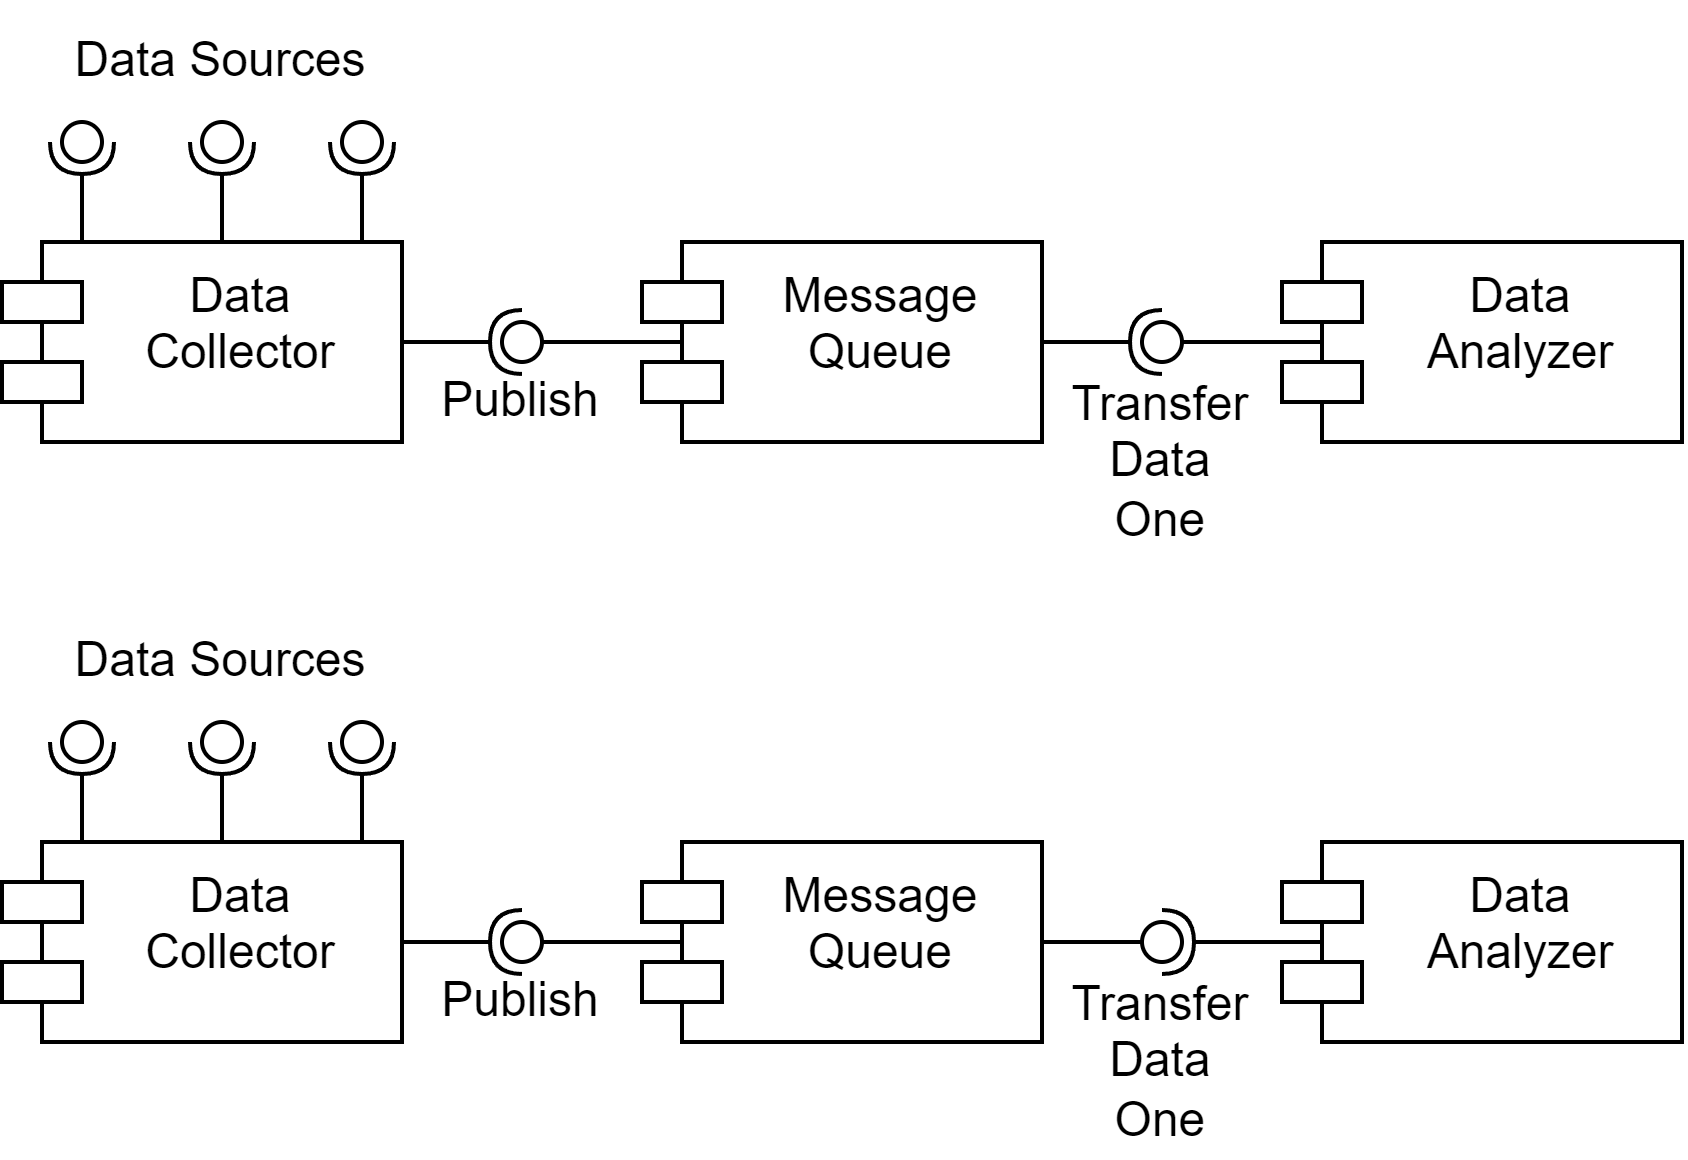
\includegraphics[width=0.75\linewidth]{images/da.png}
\end{figure}
\begin{enumerate}
    \item What is the difference between the two?
    \item Define two sequence diagrams that describe how data flow through the system in the two versions of the architecture. 
    \item Assume that the components of your system offer the following availability: \texttt{DataCollector} (0.99), \texttt{MessageQueue (0.9999)}, and \texttt{DataAnalyzer} (0.995). 
        Provide an estimation of the total availability of your system (you can provide a raw estimation of the availability without computing it completely).
    \item Assuming that you wanted to improve this total availability by exploiting replication, which component(s) would you replicate?
\end{enumerate}

\paragraph*{Solution}
\begin{enumerate}
    \item In the second case, the \texttt{MessageQueue} does not actively push the data to the \texttt{DataAnalyzer}, but it offers interface TransferData2 so that the \texttt{DataAnalyzer} can pull data as soon as it is ready to process them. 
        Also in this case, both a batch or a per data approach is possible. 
        The rest of the system behaves as first one.
    \item The sequence diagram compatible with the first component diagram is as follows: 
        \begin{figure}[H]
            \centering
            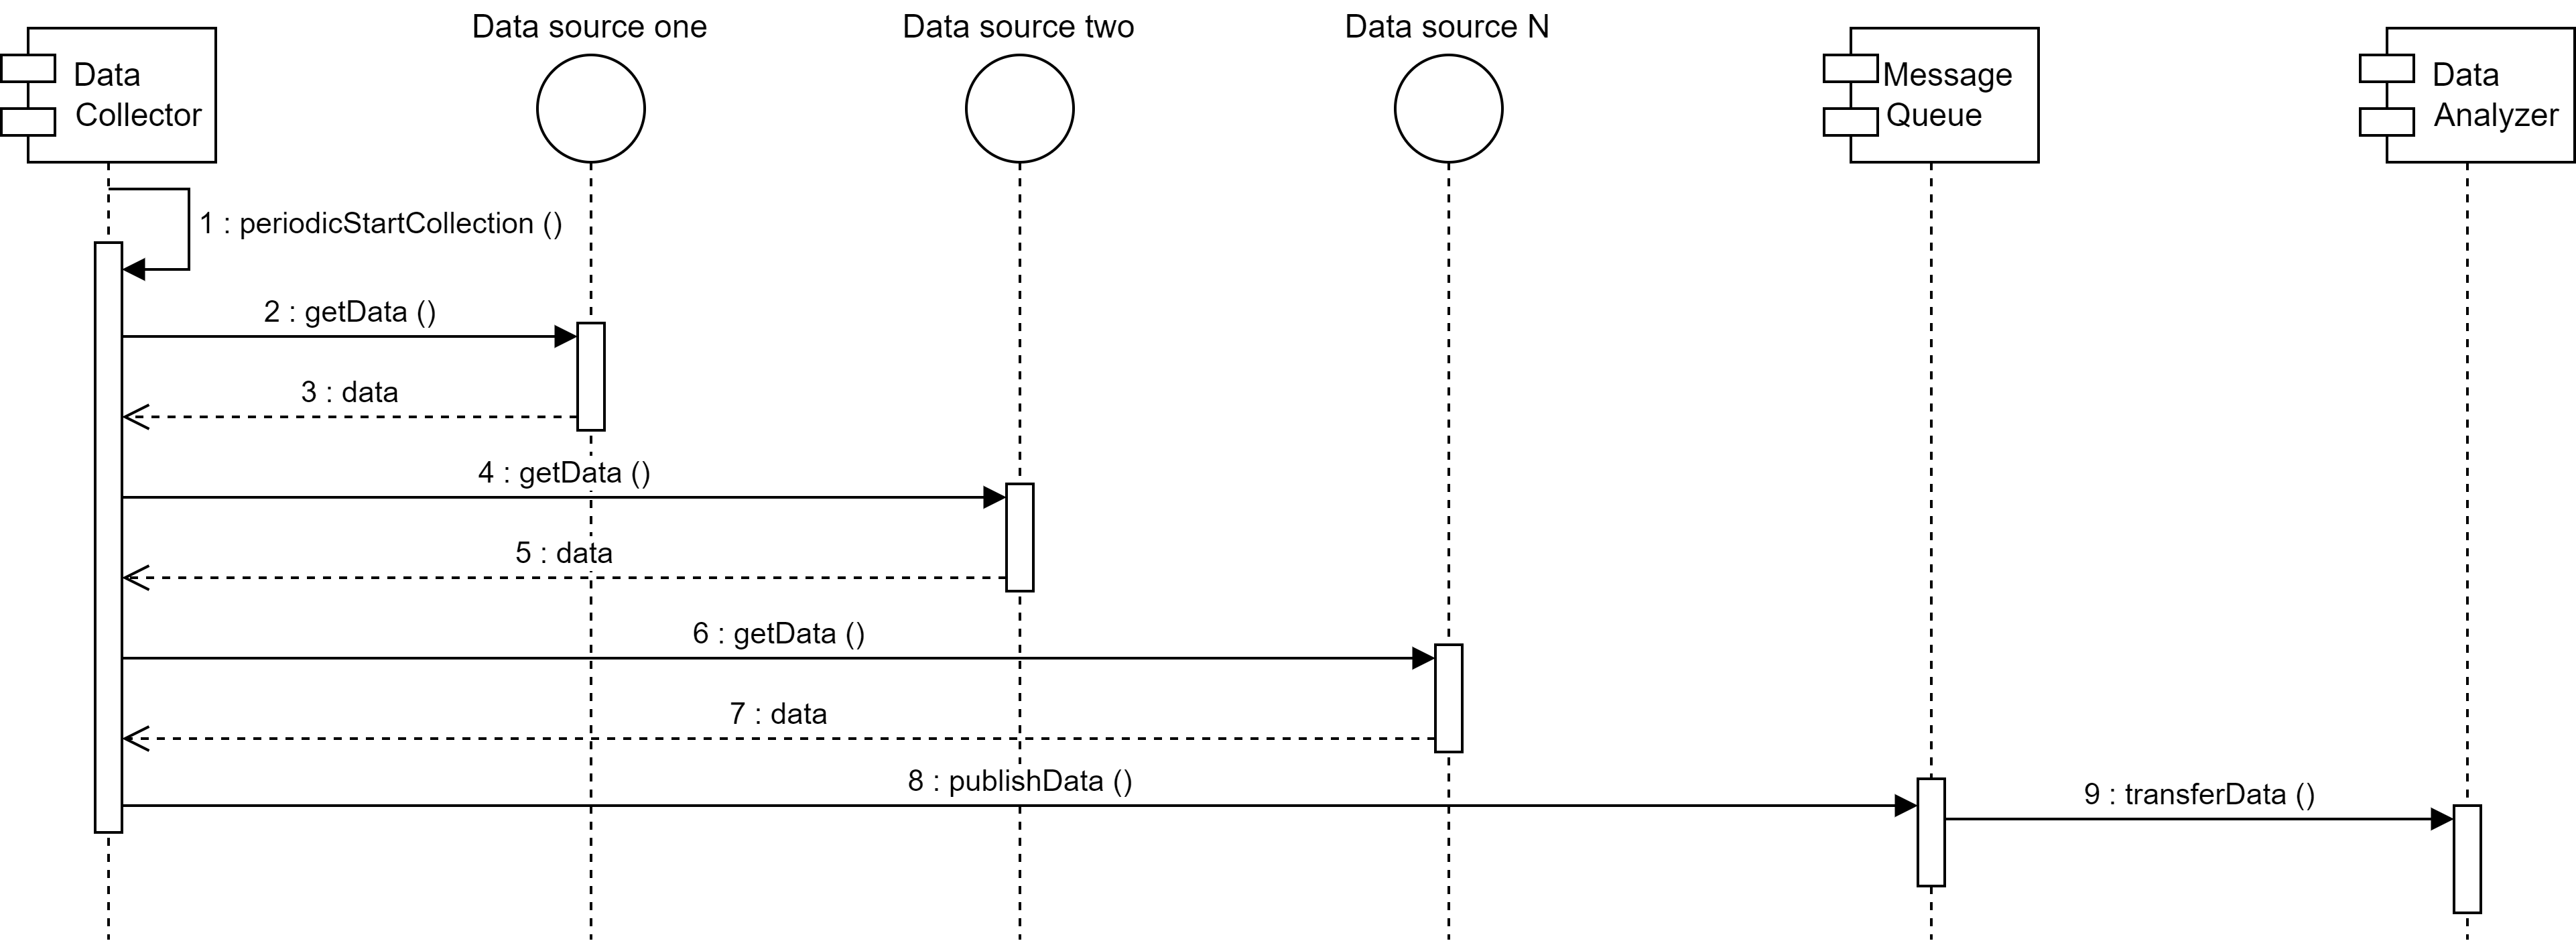
\includegraphics[width=0.9\linewidth]{images/sd3.png}
        \end{figure}
        And the sequence diagram compatible with the second component diagram is as follows: 
        \begin{figure}[H]
            \centering
            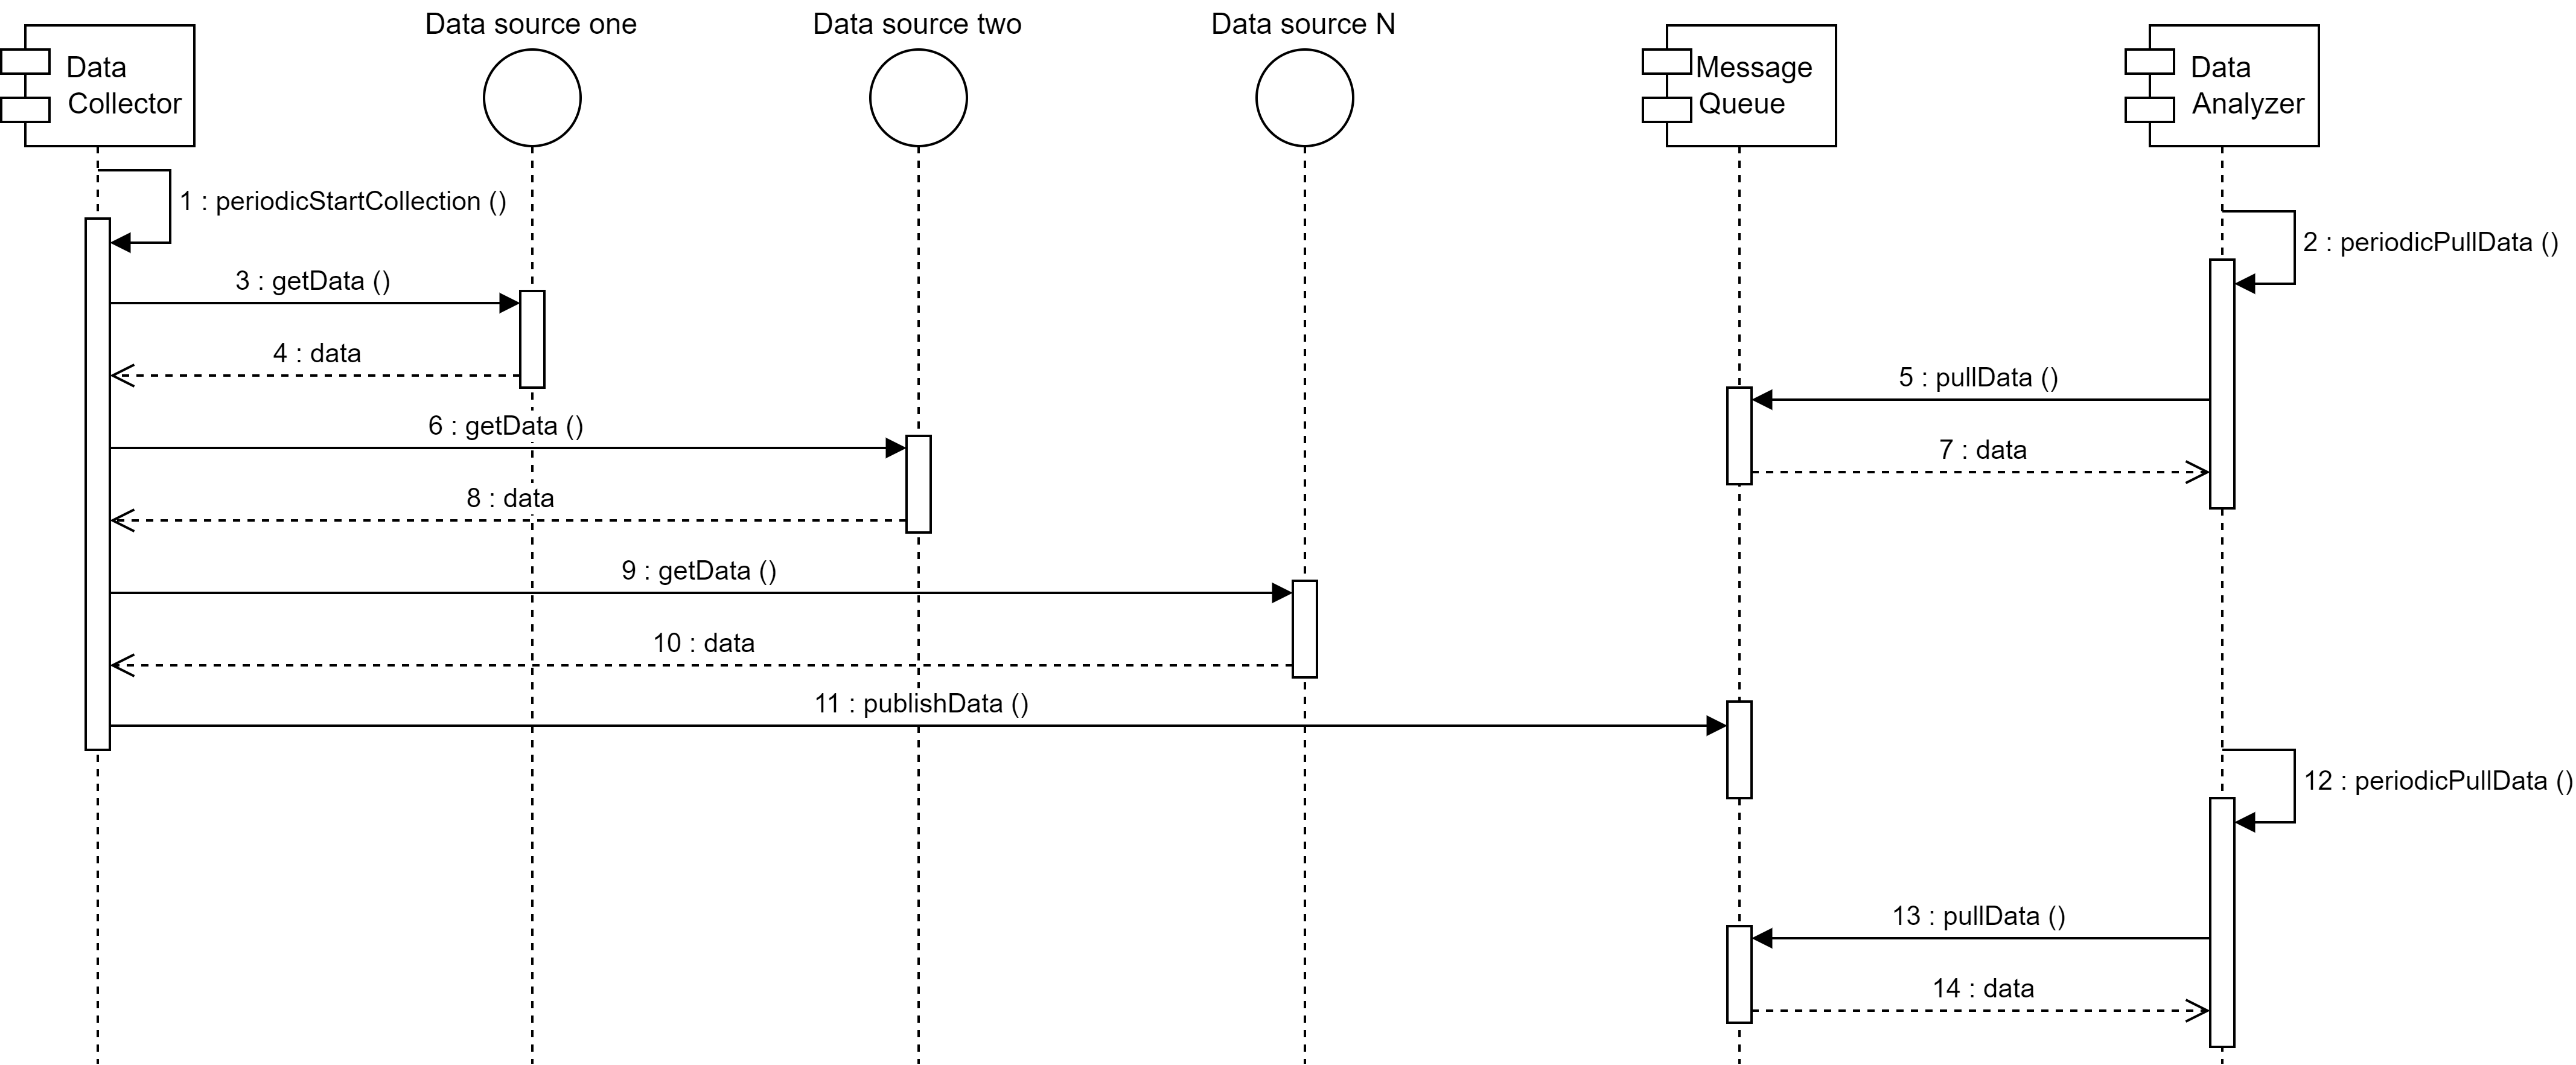
\includegraphics[width=0.9\linewidth]{images/sd4.png}
        \end{figure}
    \item Data flow through the whole chain of components to be processed. 
        Thus, we have a series of component.
        In this scenario, the total availability of the system is determined by the weakest element, that is, the \texttt{DataCollector}: 
        \[A_{\text{Total}} = 0.99 \cdot 0.9999 \cdot 0.995 = 0.985\]
    \item  If we parallelize \texttt{DataCollector} by adding a new replica, we can achieve the following availability:
    \[(1-(1-0.99)\cdot 2) \cdot 0.9999 \cdot 0.995 = 0.995\]
    If we increase the number of \texttt{DataCollector} replica, we do not achieve an improvement as the weakest component becomes the \texttt{DataAnalyzer}.
    We can parallelize this component as well to further improve the availability of our system.
\end{enumerate}